%% 
%% Copyright 2007-2020 Elsevier Ltd
%% 
%% This file is part of the 'Elsarticle Bundle'.
%% ---------------------------------------------
%% 
%% It may be distributed under the conditions of the LaTeX Project Public
%% License, either version 1.2 of this license or (at your option) any
%% later version.  The latest version of this license is in
%%    http://www.latex-project.org/lppl.txt
%% and version 1.2 or later is part of all distributions of LaTeX
%% version 1999/12/01 or later.
%% 
%% The list of all files belonging to the 'Elsarticle Bundle' is
%% given in the file `manifest.txt'.
%% 
%% Template article for Elsevier's document class `elsarticle'
%% with harvard style bibliographic references

\documentclass[preprint,12pt,authoryear]{elsarticle}
%% Use the option review to obtain double line spacing
%% \documentclass[authoryear,preprint,review,12pt]{elsarticle}

%% Use the options 1p,twocolumn; 3p; 3p,twocolumn; 5p; or 5p,twocolumn
%% for a journal layout:
%% \documentclass[final,1p,times,authoryear]{elsarticle}
% \documentclass[final,1p,times,twocolumn,authoryear]{elsarticle}
%% \documentclass[final,3p,times,authoryear]{elsarticle}
% \documentclass[final,3p,times,twocolumn,authoryear]{elsarticle}
%% \documentclass[final,5p,times,authoryear]{elsarticle}
%% \documentclass[final,5p,times,twocolumn,authoryear]{elsarticle}

\usepackage{amsmath}
\usepackage{amsfonts}
\usepackage{amssymb}
\usepackage[utf8]{inputenc}
\usepackage{url,hyperref,lineno,microtype,subcaption}
\usepackage{color,tensor,multirow,siunitx}
\usepackage[onehalfspacing]{setspace}
\usepackage{makecell}
\renewcommand{\cellalign}{cl}
\usepackage{caption}
\usepackage{lipsum}
\captionsetup[figure]{name=Fig., labelfont=bf}
\captionsetup[table]{name=Table, labelfont=bf}

\renewcommand{\cellalign}{cl}

\newcommand{\ds}{\displaystyle}
\newcommand{\nl}{\ \\ }
\newcommand{\ud}{\textrm{ d}}
\newcommand{\bs}{\bigskip}

\newcommand{\bu}{\mathbf{u}}
\newcommand{\bv}{\mathbf{v}}
\newcommand{\bx}{\mathbf{x}}
\newcommand{\be}{\mathbf{e}}
\newcommand{\bb}{\mathbf{b}}
\newcommand{\bk}{\mathbf{k}}
\newcommand{\bn}{\mathbf{n}}
\newcommand{\bR}{\mathbf{R}}

\definecolor{orange}{rgb}{1.0, 0.46, 0.09}
\definecolor{red}{rgb}{1,0,0}
\definecolor{blue}{rgb}{0,0,0.8}
\definecolor{green}{rgb}{0,0.5,0}
\newcommand{\emphc}[1]{\emph{\textcolor{red}{#1}}}
\newcommand{\hycom}{\textsc{hycom} }
\newcommand{\ie}{{\it i.e.}\ }
\newcommand{\eg}{{\it e.g.}\ }
\newcommand{\UV}{\mathbf{U}}
\newcommand{\todo}[1]{\textcolor{red}{TO DO: #1}}
%\newcommand{\modif}[1]{\textcolor{blue}{#1}}
% \renewcommand{\familydefault}{\sfdefault}

\journal{Marine Pollution Bulletin}

\begin{document}

\begin{frontmatter}

    %% Title, authors and addresses

    %% use the tnoteref command within \title for footnotes;
    %% use the tnotetext command for theassociated footnote;
    %% use the fnref command within \author or \affiliation for footnotes;
    %% use the fntext command for theassociated footnote;
    %% use the corref command within \author for corresponding author footnotes;
    %% use the cortext command for theassociated footnote;
    %% use the ead command for the email address,
    %% and the form \ead[url] for the home page:
    %% \title{Title\tnoteref{label1}}
    %% \tnotetext[label1]{}
    %% \author{Name\corref{cor1}\fnref{label2}}
    %% \ead{email address}
    %% \ead[url]{home page}
    %% \fntext[label2]{}
    %% \cortext[cor1]{}
    %% \affiliation{organization={},
    %%            addressline={}, 
    %%            city={},
    %%            postcode={}, 
    %%            state={},
    %%            country={}}
    %% \fntext[label3]{}

    \title{Potential origin of the Stony coral tissue loss disease}%Impacts of Hurricane Irma (2017) on ocean transport processes}

    %% use optional labels to link authors explicitly to addresses:
    %% \author[label1,label2]{}
    %% \affiliation[label1]{organization={},
    %%             addressline={},
    %%             city={},
    %%             postcode={},
    %%             state={},
    %%             country={}}
    %%
    %% \affiliation[label2]{organization={},
    %%             addressline={},
    %%             city={},
    %%             postcode={},
    %%             state={},
    %%             country={}}

    \author[eli]{Thomas Dobbelaere\corref{corr}}
    \ead{thomas.dobbelaere@uclouvain.be}
    %\author[rsmas]{Milan Curcic}
    %\author[cimas,aoml]{Matthieu Le H\'enaff}
    \author[eli,immc]{Emmanuel Hanert}
    \cortext[corr]{Corresponding author}

%    \affiliation[eli]{
%        organization={Eath and Life Institute (ELI), UCLouvain},
%        % addressline={}, 
%        city={Louvain-la-Neuve},
%        % postcode={1348}, 
%        % state={},
%        country={Belgium}
%    }
%    \affiliation[rsmas]{
%        organization={Rosenstiel School of Marine and Atmospheric Sciences (RSMAS), University of Miami},
%        % addressline={}, 
%        city={Coral Gables},
%        % postcode={1348}, 
%        state={Florida},
%        country={USA}
%    }
%    \affiliation[cimas]{
%        organization={Cooperative Institute for Marine and Atmospheric
%        Studies (CIMAS), University of Miami},
%        % addressline={}, 
%        city={Miami},
%        % postcode={1348}, 
%        state={Florida},
%        country={USA}
%    }
%    \affiliation[aoml]{
%        organization={Atlantic Oceanographic and Meteorological Laboratory
%        (AOML), NOAA},
%        % addressline={}, 
%        city={Miami},
%        % postcode={1348}, 
%        state={Florida},
%        country={USA}
%    }
    \affiliation[immc]{
        organization={Institute of Mechanics, Materials and Civil Engineering (IMMC), UCLouvain},
        % addressline={}, 
        city={Louvain-la-Neuve},
        % postcode={1348}, 
        % state={},
        country={Belgium}
    }

    \begin{abstract}
        \lipsum[1-2]
        % For about six years, the Florida Reef Tract (FRT) has been experiencing an outbreak of the Stony Coral Tissue Loss Disease (SCTLD). Although the epicenter of the propagation of the disease has been identified off the coast of Miami-Dade County in 2014, the origin and identity of the agent responsible for the initiation of the epidemic remain unknown. A potential scenario is that this agent was transported to the first-affected coral colonies within material driven by currents. The goal of this preliminary study is therefore to identify the potential sources of such material. Backward and forward particle tracking from May to September 2014 suggested that fine matters suspended in the water column generated by phase III of the expansion of Port of Miami (November 2013 - March 2017) might have been transported south, to the first-identified diseased colonies. However, sediment modeling showed no sediment transport south to the dredged channel during our simulated period. An extension of the simulated period is therefore required to determine whether hydrodynamics allowed sediments to reach the first-affected colonies prior to May 2014. Besides, the modeled impact of sediments on the reefs located north to the dredged channel suggest that the SCTLD outbreak might have been initiated north to the reefs where it was first observed in 2014. Further propagation studies would assess the feasibility of disease transmission from the north to the south of the dredged channel.
    \end{abstract}

    %%Graphical abstract
    % \begin{graphicalabstract}
    % %\includegraphics{grabs}
    % \end{graphicalabstract}

    %Research highlights
    % \begin{highlights}
    %     \item The coupled SLIM+SWAN model correctly reproduced the hydrodynamics and waves during Irma.
    %    \item Wave radiation stress increased currents by up to 1 m/s during Irma.
	%    \item Wave radiation stress gradients were the largest on the shelf break and over reefs. 
	%   \item Waves could deflect drifting particles by up to 20 km during the hurricane.
	%  \item The Stokes drift had an impact on transport 4 times larger than the wave radiation stress.
    % \end{highlights}

    \begin{keyword}
        Stony coral tissue loss disease \sep sediments \sep Port of Miami \sep Coastal modeling \sep 
    %% keywords here, in the form: keyword \sep keyword

    %% PACS codes here, in the form: \PACS code \sep code

    %% MSC codes here, in the form: \MSC code \sep code
    %% or \MSC[2008] code \sep code (2000 is the default)

    \end{keyword}

\end{frontmatter}

\linenumbers

\section{Introduction}

%  PARAGRAPH DISEASES IN GENERAL
Coral diseases are a major threat to coral reef ecosystems and have led to significant declines in coral cover especially within the Caribbean region \citep{richardson1998coral, sutherland2004disease, aronson2001white, harvell2007coral, brandt2009dynamics}. One of the latest and the most damaging outbreak to date in Florida's Coral Reef (FCR) is stony coral tissue loss disease (SCTLD) \citep{noaa2018}. First observed off the coast of Miami in 2014 by \cite{precht2016unprecedented}, the disease has since spread through the entirety of FCR \citep{muller2020spatial,dobbelaere2022} and has been observed in several territories of the Caribbean \citep{kramer2019map, meiling2021variable, estrada2021effects,heres2021ecological}. Although the causative agent of the disease remains unknown, hydrodynamics are likely to play an important role in its propagation as both modeling studies and ex situ experiments show evidence of waterborne disease transmission \citep{aeby2019pathogenesis,dobbelaere2020coupled,eaton2021measuring, meiling2021variable}. Furthermore, recent studies showed evidence that sediments act as vector for the SCTLD \citep{rosales2020rhodobacterales, studivan2022reef}.

% POM
SCTLD was first observed by \cite{precht2016unprecedented} near Virginia Key in September 2014, during the deepening of the Port of Miami (PoM) shipping channel, that took place between November 20, 2013 and March 16, 2015. The dredging was monitored twice-weekly at 26 monitoring stations established within the Miami-Dade County, making it one of the most complete datasets related to a dredging project \citep{gintert2019regional}. While operating in a conventional way, dredged materials were pumped from the dredge to a spider barge and then transported to the US Environmental Protection Agency designated Ocean Dredge Material Disposal Site (ODMDS) located 4.7 nautical miles offshore. However, the suction mechanism was turned off during non-conventional rock-chopping activities in order to pre-treat very hard rock contained in the Anastasia and Fort Thompson formations between December 2013 and May 2014. The Army Corps commissioned a report that provides a back-of-the-envelope estimating this practice could have resulted in up to 33 cm deposition over 874,121 m$^2$ of reef surrounding the outer entrance channel (Jocelyn Karazsia, \textit{pers. comm.}). Additionally, several studies reported that the impact of the dredging was widespread \citep{miller2016detecting}, causing the death of  $> 560,000$ corals within 0.5 km of the channel \citep{cunning2019extensive} and producing sediment plumes covering up to 11 km$^2$ of coral area within 5-10 km of the dredging \citep{barnes2015sediment}.

% SEDIMENTS
Sediments released by dredging can affect the biological functions of corals in numerous ways \citep{erftemeijer2012environmental, jones2015effects}. Increased turbidity caused by the suspended sediments reduces the light available to symbiotic zooxanthellae, leading to reduced coral cover and growth, while increased sedimentation can cause smothering or burial of coral polyps \citep{erftemeijer2012environmental}. Furthermore, sedimentation and turbidity can significantly reduce larval recruitment by inhibiting settlement and reducing larval survival in the water column \citep{jones2015effects}. These effects are stronger with fine-grained sediments, as they cause a stronger light reduction \citep{fourney2017additive}. Additionally, fined-grained sediments such as silts have high nutrient contents, which can lead to an increased microbial activity, eventually causing anoxic conditions in the immediate vicinity of corals \citep{weber2012mechanisms}. As they release finer sediments over significantly longer periods than natural events such as hurricanes, dredging activities can thus be more harmful to corals and reef habitat compared to other types of sedimentation \citep{cunning2019extensive}.

% ON ENTRE DANS LE VIF DU SUJET
Nonetheless, \cite{gintert2019regional} argued that the reported coral mortality during the dredging project was dominated by the regional outbreak of SCTLD. Further, the study suggested that the onset of the disease might have been linked to a leaking discharge pipe of the Miami Central District Municipal Wastewater Treatment Plant located off Virginia Key. However, as sediments can act as vector for SCTLD \citep{studivan2022reef}, there is also a possibility that the causative agents of the disease was transported to the monitoring site of Virginia Key on sediments released by the dredging. This possibility can be evaluated using a bio-physical model simulating the transport of sediments produced during the dredging project. As coastal reef ecosystems are characterized by the complex topography of the coastline and the presence of islands, reefs and artificial structures, such a model would require high spatial resolution to accurately represent the transport of sediments at reef-scale. In this context, unstructured-mesh models are best suited, as they can easily adapt to the topography \citep{fringer2019future} and can capture small-scale circulation features around reefs and islands \citep{lambrechts2008multi, figueiredo2013synthesizing}.

The goal of this study is therefore to simulate the trajectories of the sediments released during the entirety of the deepening of the PoM shipping channel using a high-resolution hydrodynamic model coupled with a sediment transport model. Specifically, we will attempt to answer the following questions: (1) Which reefs were impacted by the dredging ? (2) Is the impact on these reefs consistent with the observed timing of the onset of SCTLD ? 

% === METHODS === %
\section{Methods}

\begin{figure}
    \centering
    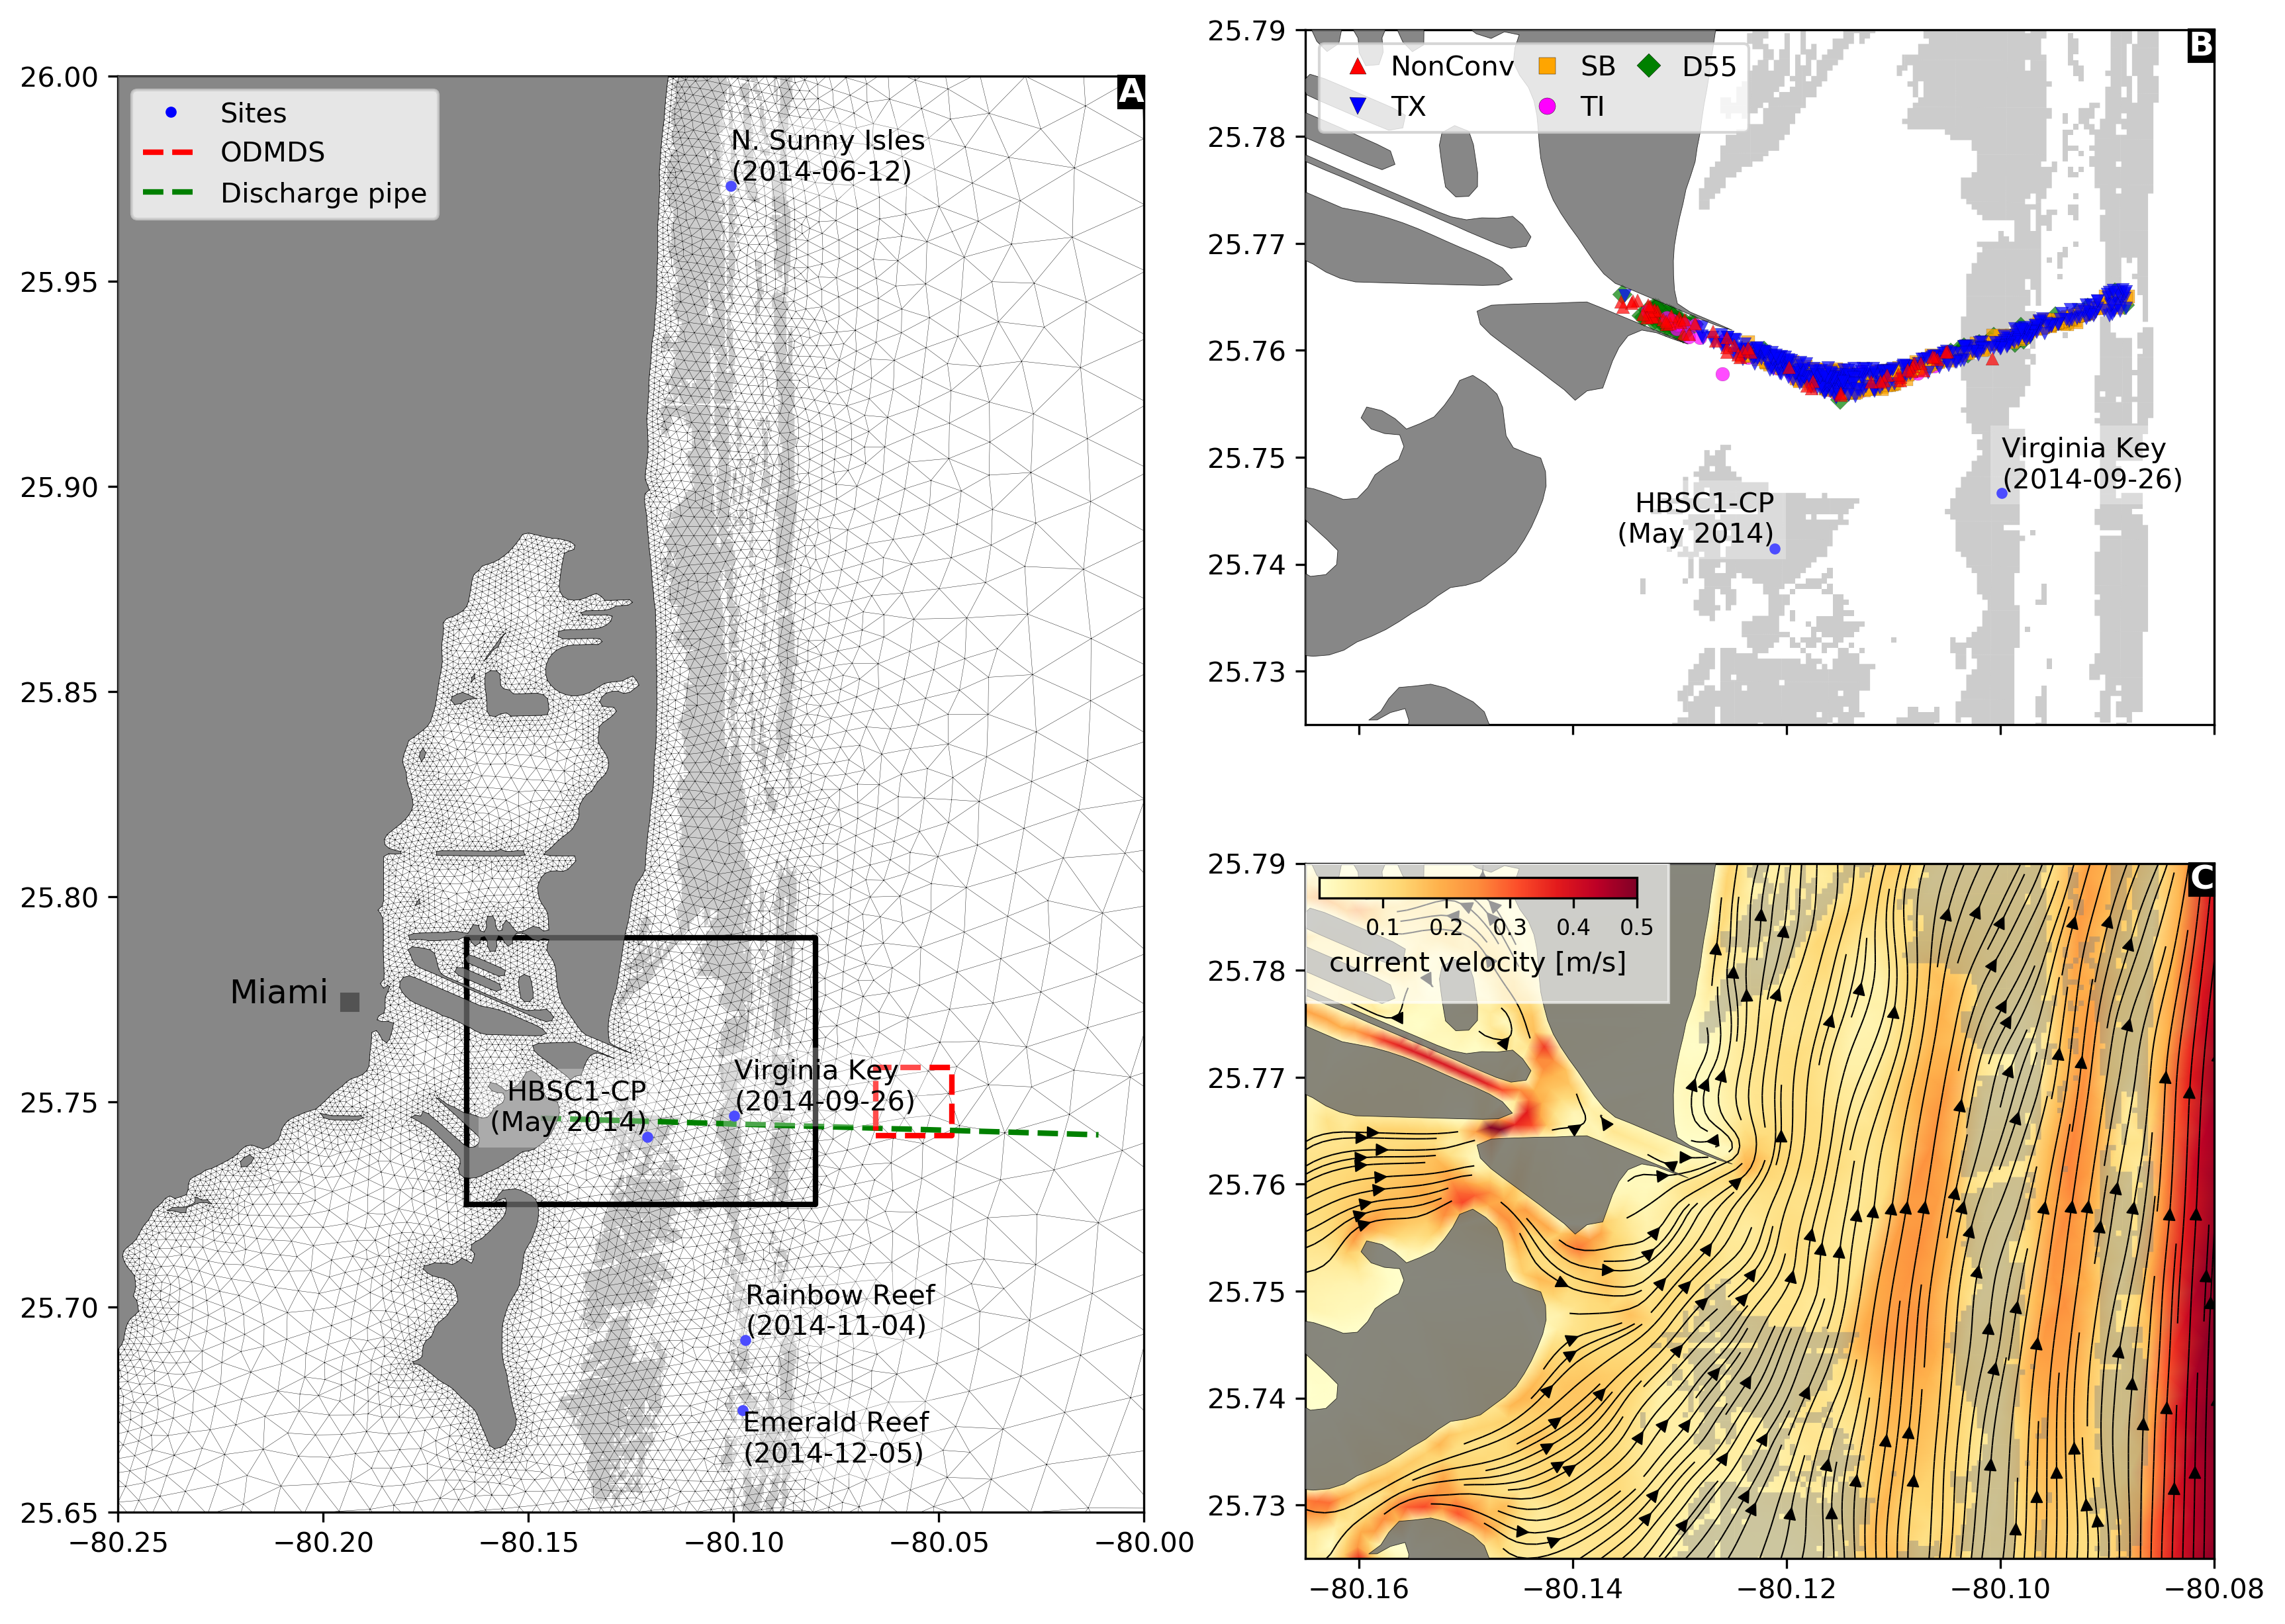
\includegraphics[width=\textwidth]{figures/fig_mesh_onset.png}
    \caption{\textbf{A}: SLIM mesh near the dredged channel. Elements have a characteristic length of 100 m over reefs (in light grey) and along the coasts (in dark gray). The monitoring sites considered in the present study are shown by blue dots. The date where SCTLD was first observed at these sites is given inside parentheses. Ocean Dredge Material Disposal Site (ODMDS) is shown by a red dashed lines. \textbf{B}: Close up view of the dredged channel. The locations of the different types of dredging that took place during the expansion of PoM are shown by colored markers. \textbf{C:} Snapshot of the modeled currents in the vicinity of the dredged channel. Small-scale flow features such as the acceleration of currents between reefs and between islands are well captured by the model.}
    \label{fig:onset_mesh}
\end{figure}

The hydrodynamics over the entirety of FCR was modeled using the high resolution unstructured-mesh model SLIM\footnote{\url{ https://www.slim-ocean.be}}, which has already been extensively validated in the area \citep{frys20,dobbelaere2020coupled,dobbelaere2022}. SLIM uses an unstructured mesh whose resolution can be locally increased in order to accurately represent fine-scale flow features. The mesh used in this study was built following the same methodology as \cite{dobbelaere2022}, with a local refinement near PoM and in the Bay of Biscayne to achieve a resolution of 100 m in the vicinity of the dredged channel (Fig. \ref{fig:onset_mesh}A). It was made up of approximately $3.5\times 10^5$ triangles and was generated with the seamsh\footnote{\url{https://pypi.org/project/seamsh/}} Python library, which is based on the the open-source mesh generator GMSH \citep{geuzaine2009gmsh}. The model was run between October 15, 2013 and September 26, 2014 to cover the whole dredging period prior to the first observation of SCTLD by \cite{precht2016unprecedented}. Figure \ref{fig:onset_mesh}C depicts how a 100-m spatial resolution mesh simulated fine-scale details of the ocean currents, such as the accelerations between reefs and between islands.

The transport of sediments released from the channel was then modeled using a Lagrangian particle tracking model, forced by SLIM velocity field. The sediment model is inspired by the Particle Transport Model (PTM), developed by the US Army Corps of Engineers \citep{macdonald2006ptm}. In this model, particles undergo a combination of horizontal and vertical motions. The vertical is mostly driven by gravity, with heavier particles sinking faster. Once sedimented, particles can be resuspended when shear stress exceed the critical Schields parameter, as parameterized by \cite{soulsby1997threshold}. The horizontal motion of the suspended particles is dervued from the 2D model velocity by assuming a vertical log profile, following a quasi-3D approach. When sediment particles enter the near-bed zone, their horizontal velocity is greatly reduced and sediments are transported with the bedload.

As sediment dispersion is dependent on the grain size, we modeled the dispersal of five classes of sediments to represent to impact of fine- to coarse-grained particles: ($i$) 5-50 $\mu$m, ($ii$) 50-100 $\mu$m, ($iii$) 100-200 $\mu$m, ($iv$) 200-300 $\mu$m, and ($v$) 300-400 $\mu$m. We performed a  different simulation for each class, with the grain size randomly drawn from a uniform distribution over the corresponding size range. The density of each sediment particle was derived from their size using the formula of \cite{hamilton1982sound}. Furthermore, all particles were differentiated based on the dredge that produced them. Five types of dredge were considered in our modeling study (Fig. \ref{fig:onset_mesh}B): ($a$) Texas cutterhead (TX), ($b$) non-conventional dredging, \ie TX with suction mechanism turned off (NonConv), ($c$) Spider Barge (SB), ($d$) Terrapin Island hopper (TI), and ($e$) Dredge 55 clamshell (D55).

We had data about the date, location and type of all dredging operations performed during expansion of PoM (Fig. \ref{fig:onset_mesh}B). In the absence of information about the exact time of the dredging, sediment particles were released from the dredging location during a whole day at a rate of 80 particles/hour in the model. To account for the motion of spider barges between the dredging site and disposal site, particles were released every 500 m along a straight line joining the dredging location to the ODMDS (see Fig. \ref{fig:onset_mesh}A) for every dredging operation labelled as SB. 

\todo{write about validation using presence-absence of plume ?}

We evaluated the impact of dredging at five different sites. Four sites are reefs where disease was reported in 2014 by \cite{precht2016unprecedented}. The fifth site is monitoring station HBSC1-CP, where signs of disease were reported in May 2014 (Fig. \ref{fig:onset_mesh}A). The impact of dredging was assessed by counting the number of sediment particles originating from each dredging that were transported within 500 m of all five site. This number was then divided by the total number of sediment particles released by each type of dredge. Larger values of this indicator would suggest a greater impact of a given type of dredging at a given monitoring sites.

Furthermore, as previous studies showed evidence of waterborne transmission of SCTLD \citep{aeby2019pathogenesis, dobbelaere2020coupled,eaton2021measuring, meiling2021variable}, there is a possibility that the disease propagated to Virginia Key another diseased reefs affected prior to September 2014. To evaluate this possibility, we computed monthly disease connectivity matrices following the methodology of \cite{dobbelaere2020coupled} during our simulated period. These connectivity matrices can be interpreted as large graphs whose vertices are sub-areas of reefs and whose edges represent disease connectivity pathways. Evaluating the possibility of disease propagation from one reef to another is therefore equivalent to evaluating the presence of paths connecting sub-reef areas if these two reefs in the network. As computing all possible paths is not computationally tractable, we limited ourselves to the computation of shortest paths from any given reefs to the Virginia Key monitoring site. This was performed using the function \texttt{get\_all\_shortest\_paths} of the Python \texttt{python-igraph} package \citep{csardi2006igraph}. Such function requires the definition of a weight $w_{ij}$ for the edge connecting reef $i$ to reef $j$. We chose $w_{ij} = 1-\tilde{C}_{ij}$, where $\tilde{C}_{ij}$ is the probability of disease propagation from reef $i$ to reef $j$, so that "shorter" edges of the networks (\ie connectivity pathways with smaller weights) correspond to connections with larger disease propagation probability. The probability of a given path was then defined as the mean connection probability of the edges composing this path.
  
%%%%%%%%%%%%%%%%%%%
% --- RESULTS --- %
%%%%%%%%%%%%%%%%%%%
\section{Results}

Our sediment simulations indicate that, with the exception of site HBSC1-CP, dredging did not significantly impact the reefs located south to the channel. However, up to 50\% of the released sediment particles reached the northern site of N. Sunny Isles. These results are illustrated in Fig. \ref{fig:onset_bar} for grain sizes corresponding to silts, as such sediments are more likely to carry organic matter and have a greater impact on corals. However, the impact of dredging on N. Sunny Isles decreases with sediment size and the proportion of sediment particles reaching the site drops below 2\% for grain sizes larger than 200 $\mu$m. On the other hand, the proportion of sediment particles reaching HBSC1-CP remains between 2\% and 5\% for all grain sizes. For all grain sizes, no modeled sediment particles reached the sites of Rainbow Reef and Emerald Reef. However, some modeled particles reached Virginia Key for grain sizes larger than 100 $\mu$m . However, the impact of the dredging on Virginia Key remained limited with less than 1$\%$ of the released particles reaching the site.

\begin{figure}
    \centering
    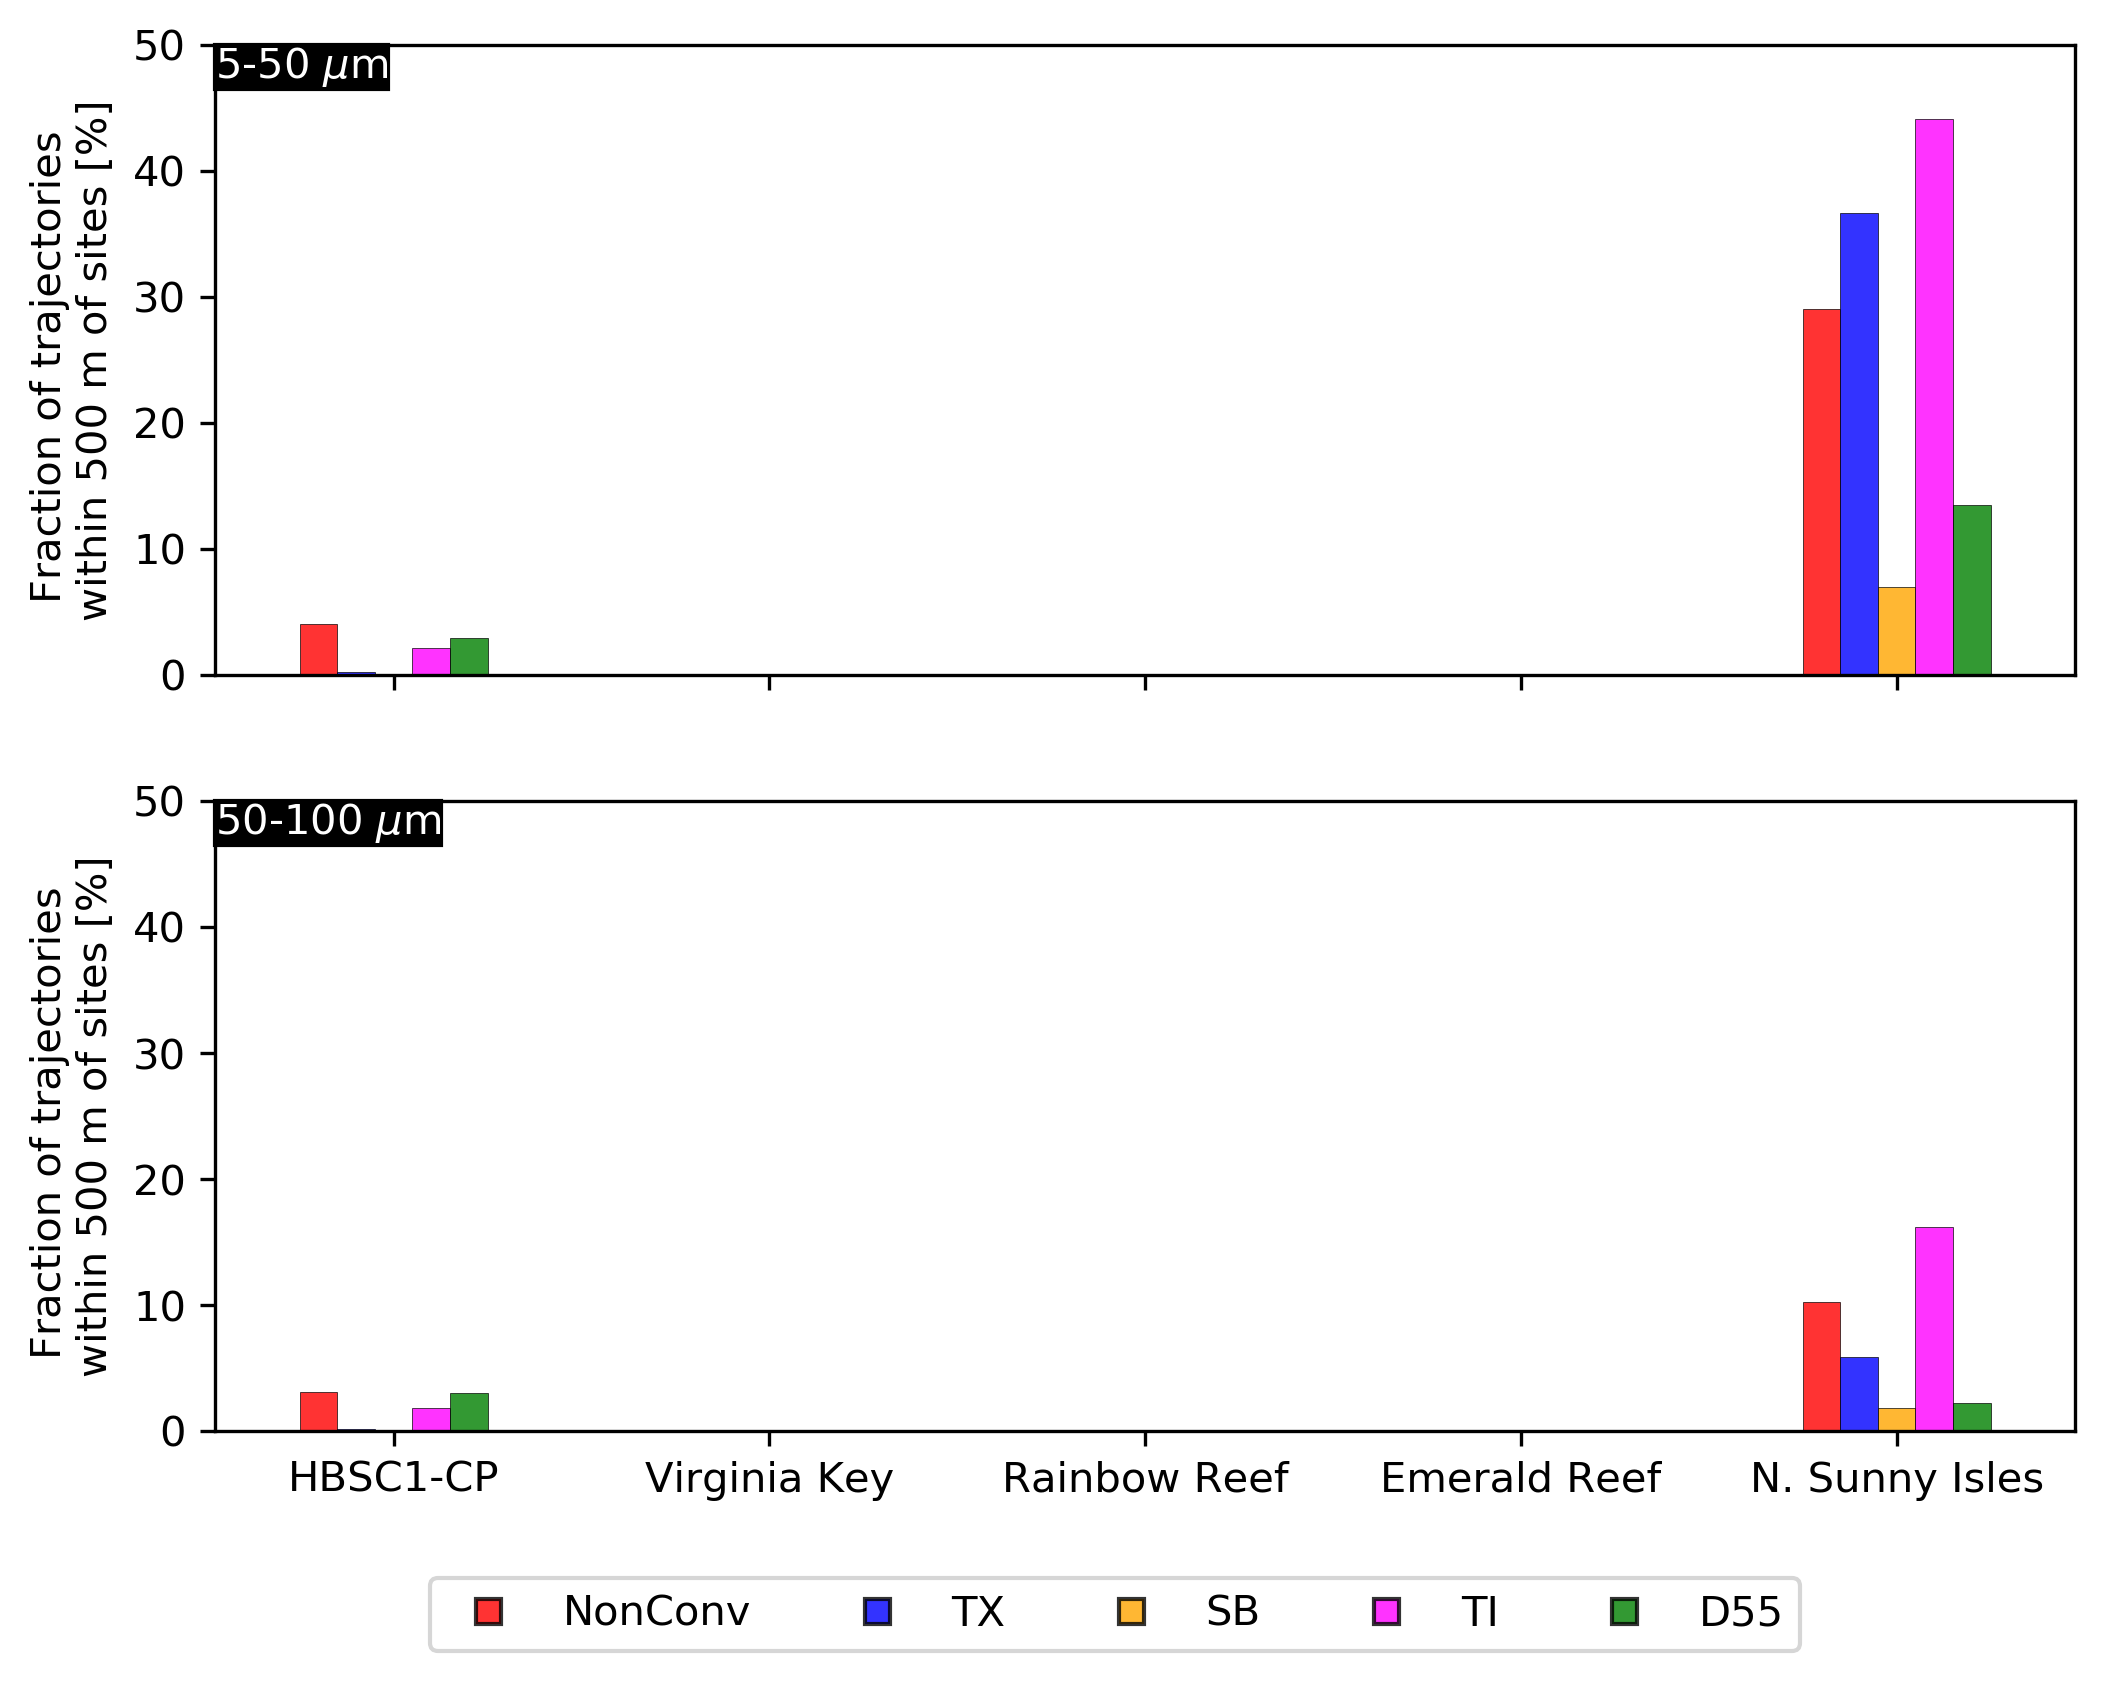
\includegraphics[width=\textwidth]{figures/aggregated_silts.png}
    \caption{Fraction of sediment particles released by each type of dredge that drifted within 500 of the monitoring sites for the grain size classes corresponding to silts: 5-50 $\mu$m (top) and 50-100 $\mu$m (bottom). With the exception of HBSC1-CP, sites located south to the dredged channel were barely impacted by the dredging. However, a significant fraction of the released sediment particles reached the northern site of N. Sunny Isles.}
    \label{fig:onset_bar}
\end{figure}

As signs of disease were observed at site HBSC1-CP in May 2014, before the first observations of SCTLD in Virginia Key in September 2014, we assessed the presence of shortest paths from HSC1-CP to Virginia Key in the modeled monthly disease connectivity networks between May and September 2014 (Fig. \ref{fig:onset_path}). We found connectivity pathways connecting the two sites during all months of May-September 2014, except July 2014. This suggests that there was a possibility of disease propagation from HBSC1-CP to Virginia Key during most of these 5 months. However, we found no direct pathway connecting the two sites. Southern intermediary reefs were systematically needed as stepping stones for the propagation of the disease. This suggests that several months might have been required for disease agents to reach Virginia Key from HBSC1-CP. Moreover, shortest paths in June, August and September 2014 had many sub-reef stepping stones in common. These similar connectivity patterns indicate favorable conditions for disease propagation over several months from HBSC1-CP to Virginia Key during this period.  

\begin{figure}
    \centering
    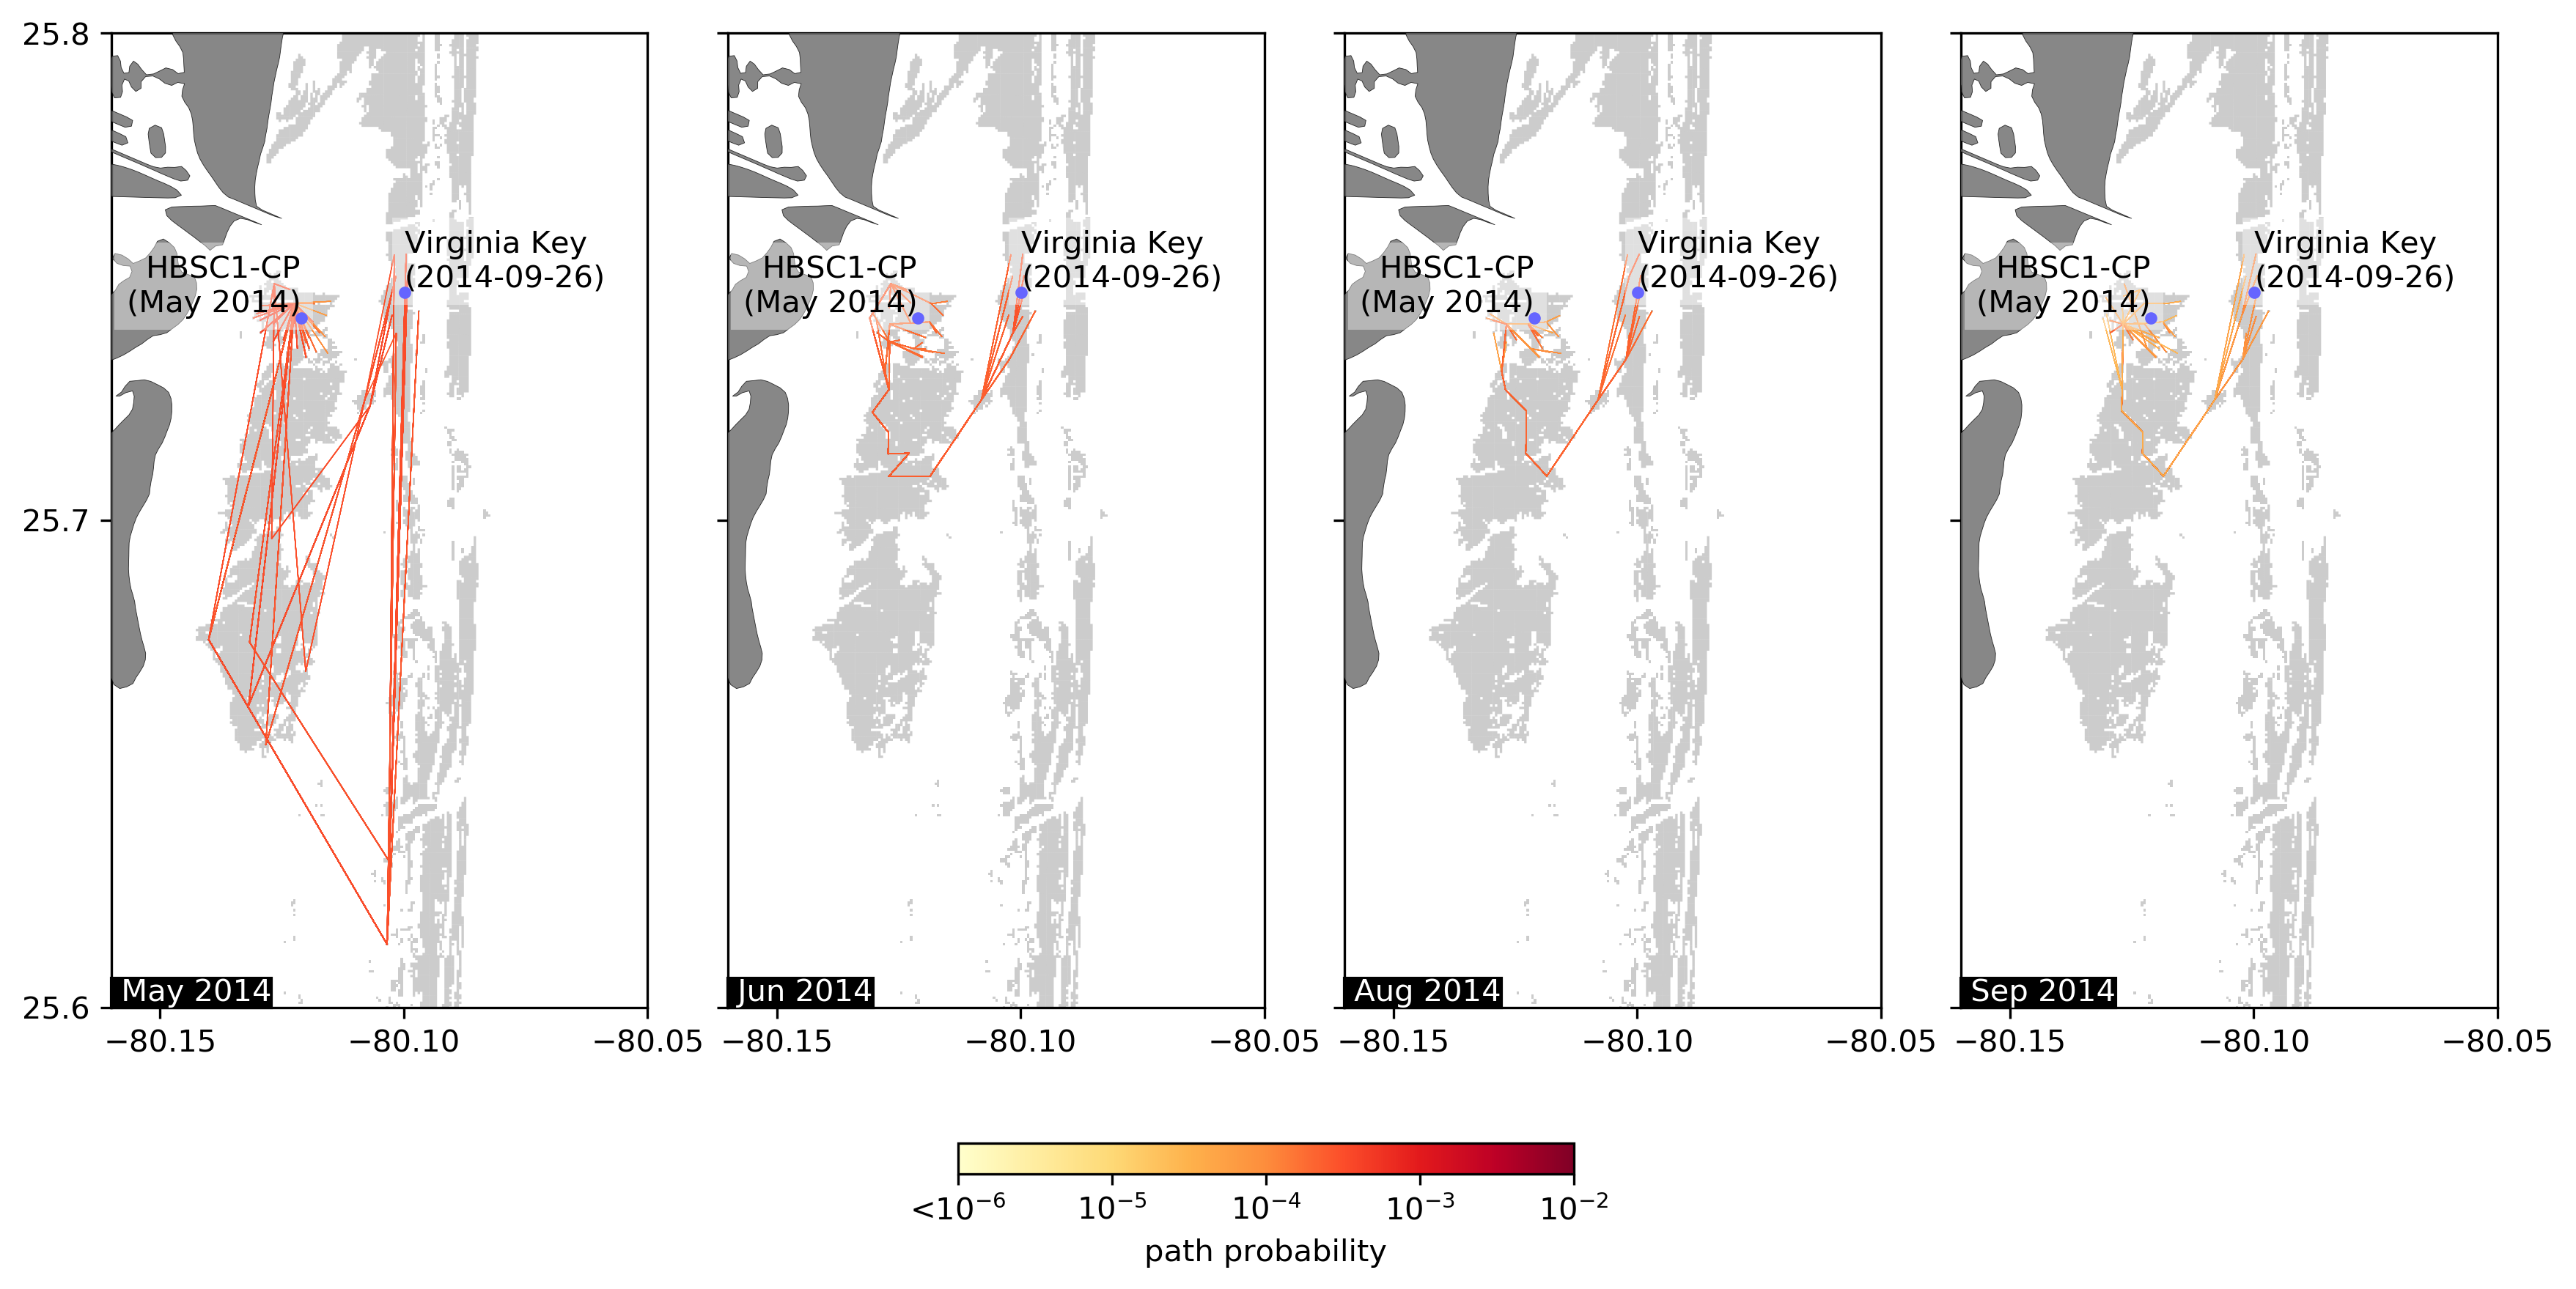
\includegraphics[width=\textwidth]{figures/fig_paths.png}
    \caption{Shortest path from HBSC1-CP to Virginia Key in the monthly disease connectivity networks between May and September 2014. July 2014 was the only month without modeled connectivity between the two sites between May and September 2014. Southern intermediary reefs were needed as stepping stones for the propagation of the disease from HBSC1-CP to Virginia Key.}
    \label{fig:onset_path}
\end{figure}

% === DISCUSSION === %
\section{Discussion}

\section{Conclusion}


\bibliographystyle{elsarticle-harv} 
\bibliography{./biblio.bib}

\end{document}
\endinput